%\documentclass{jsarticle}
\documentclass{article}

\usepackage[a4paper, margin=1in]{geometry}
\usepackage{amsmath}
\usepackage{bm}
\usepackage[usenames, dvipsnames]{xcolor}
\usepackage{url}
\usepackage[title]{appendix}

\usepackage[dvipdfmx]{graphicx}
\graphicspath{ {./images/} }

\usepackage{listings}
\lstset{
  frame=lines,
  label={lst:code_direct},
  basicstyle=\footnotesize,
  numbers=left
}

\title{グラフベースSLAM}
\date{}
\author{}

\begin{document}

\maketitle

\section{グラフベースSLAMとは}

グラフベースSLAMとはオフラインSLAMの一種で、収集した全ての観測データを用いてロボットの過去も含めた経路とランドマークの位置を修正する手法である。
本手法は時刻 $t_i$ におけるロボットの姿勢を頂点、時刻 $t_i$ での姿勢と時刻 $t_j$ での姿勢の2点間のベクトルを辺とみなして、動作辺(オドメトリなど内界センサにより得られた情報)と観測辺(レーザーレンジファインダなどの外界センサにより得られた情報)との間の誤差を全て考慮したコスト関数を最小化するロボットの経路とランドマークの位置を推測する。

\begin{figure}[h!]
  \centering
  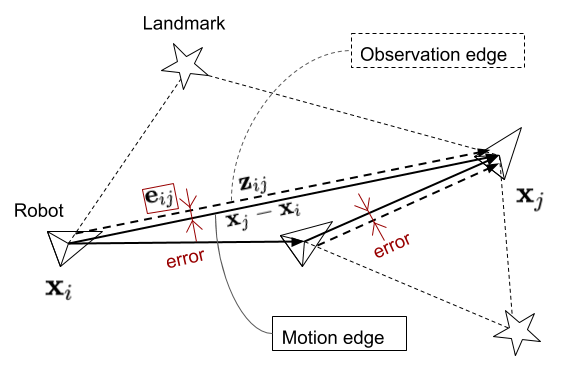
\includegraphics[width=0.8\textwidth]{1-1_error_between_edges.png}
\end{figure}

時刻 $t_i$ と時刻 $t_j$ 間での動作辺と観測辺との誤差 $\bm{e}_{ij}$ は、

\[
\bm{e}_{ij}(\bm{x}_i, \bm{x}_j) = (\bm{x}_j - \bm{x}_i) - \bm{z}_{ij}
\]

ここで $\bm{x}_i$ と $\bm{x}_j$ はそれぞれ時刻 $t_i$ と時刻 $t_j$ でのロボットの姿勢、 $\bm{z}_{ij}$ は時刻 $t_i$ と時刻 $t_j$ で同じランドマークを観測した際に得られる観測辺である。
従ってコスト関数 $F(\bm{x}_{0:t})$ は、

\[
F(\bm{x}_{0:t}) = \sum_{i,j} \bm{e}_{ij}(\bm{x}_i, \bm{x}_j)^{\mathrm{T}} \Omega_{ij} \bm{e}_{ij}(\bm{x}_i, \bm{x}_j)
\]

と、情報の正確さを表す $\Omega_{ij}$ で重み付けされた二乗誤差 $\bm{e}_{ij}^{\mathrm{T}} \bm{e}_{ij}$ (マハラノビス距離)の総和で表すことができる。
グラフベースSLAMとは、このコスト関数を最小化するロボットの経路及びランドマークの位置を探す事である。

\newpage

\section{定義}

本稿で使用する座標系と文字をいくつか定義する。

\subsection{座標系}

基準となる絶対座標系上に、ロボットの姿勢が2つ、ランドマークが1つあるとする。
ロボットは自分を原点とした車両座標系を持ち、車両前方方向をX軸、それに垂直な左手方向をY軸とする。
また、ランドマーク自身も位置だけでなく各々の角度を持っているとする。しかしそのランドマークの角度の値自体は重要ではない(後述)。

\begin{figure}[h!]
  \centering
  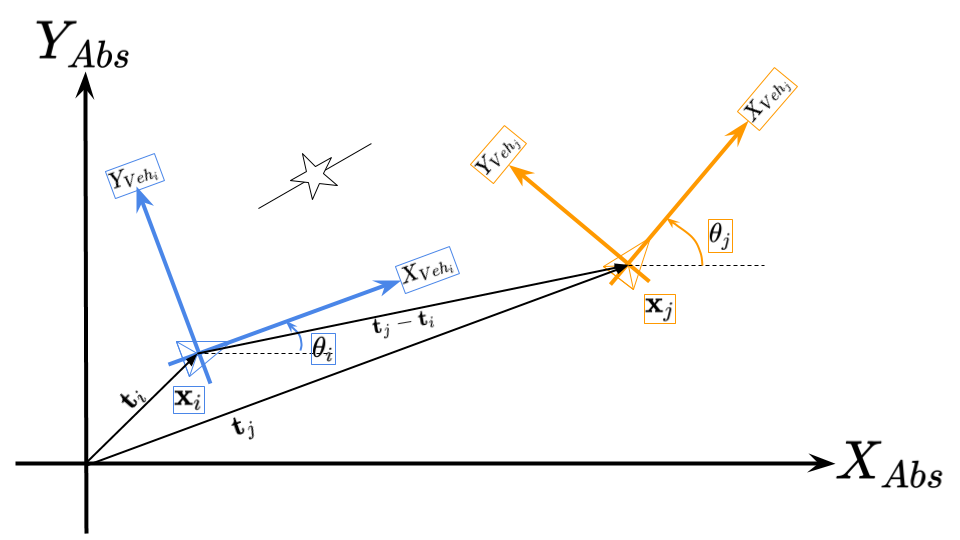
\includegraphics[width=\textwidth]{2-1_coordinate.png}
\end{figure}

\subsection{ロボットの位置ベクトル: $\bm{t}_i$}

ロボットの絶対座標系における $x_i$ 座標と $y_i$ 座標から成るベクトル。

\[
\bm{t}_i =
\left(
  \begin{array}{c}
    x_i \\
    y_i \\
  \end{array}
\right)
\]

\subsection{ロボットの姿勢ベクトル: $\bm{x}_i$}

しかしながらロボットはもう一つ、絶対座標系のX軸から車両座標系のX軸までの角度であるヨー角度というパラメータを持っている。

\[
\bm{x}_i =
\left(
  \begin{array}{c}
    \bm{t}_i \\
    \theta_i \\
  \end{array}
\right)
=
\left(
  \begin{array}{c}
    x_i \\
    y_i \\
    \theta_i \\
  \end{array}
\right)
\]

\newpage

\subsection{回転行列: $R_i$}

回転行列による座標変換は、座標系を時計回りに回転させる。特に $R_i$ は、車両$_i$座標を絶対座標に回転変換する。

\[
R_i =
\left(
  \begin{array}{ccc}
    cos\theta_i & -sin\theta_i \\
    sin\theta_i &  cos\theta_i \\
  \end{array}
\right)
\]

\begin{figure}[h!]
  \centering
  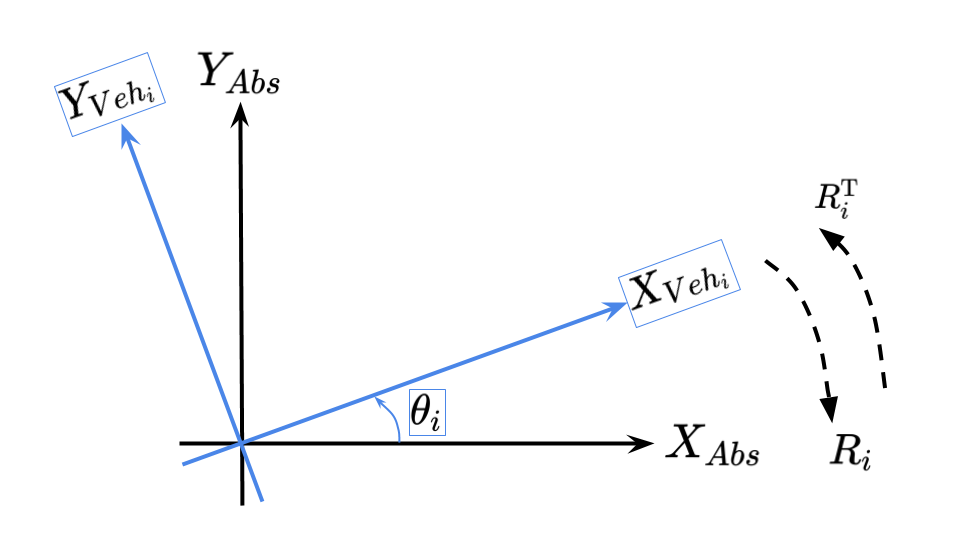
\includegraphics[width=0.6\textwidth]{2-2_rotation_matrix.png}
\end{figure}

\subsection{姿勢表現行列: $X_i$}

本稿では、回転行列 $R_i$ と位置ベクトル $t_i$ から構成される姿勢表現行列によってロボットの姿勢を表すこととする。

\[
X_i =
\left(
  \begin{array}{ccc}
    R_i & \bm{t}_i \\
     00 &          1 \\
  \end{array}
\right)
=
\left(
  \begin{array}{ccc}
    cos\theta_i & -sin\theta_i & x_i \\
    sin\theta_i &  cos\theta_i & y_i \\
              0 &            0 &   1 \\
  \end{array}
\right)
\]

\begin{figure}[h!]
  \centering
  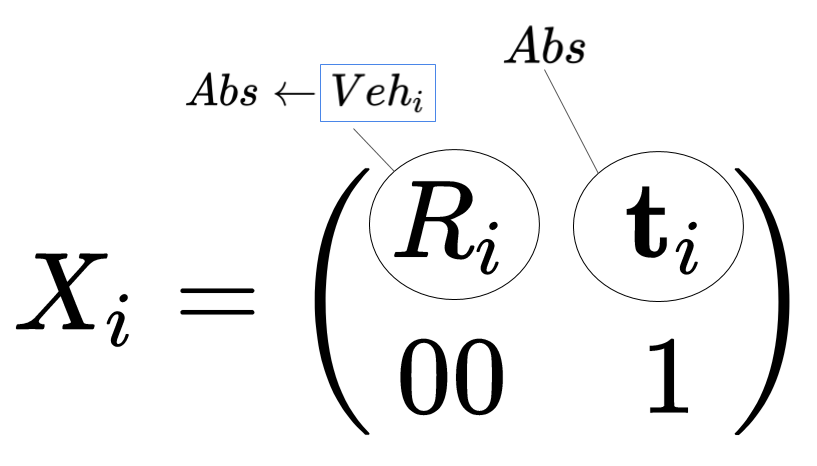
\includegraphics[width=0.4\textwidth]{2-3_pose_representation_matrix.png}
\end{figure}

姿勢行列が自身の車両座標系から絶対座標系に座標変換するのに対し、
姿勢表現行列の逆行列は絶対座標系から自身の車両座標系に座標変換することを意味する。
特に $X_i^{\mathrm{T}}$ は絶対座標系から車両$_i$座標系に変換する。

\[
X_i^{-1} =
\left(
  \begin{array}{ccc}
    R_i^{\mathrm{T}} & -R_i^{\mathrm{T}}\bm{t}_i \\
                  00 &                           1 \\
  \end{array}
\right)
\]

\begin{figure}[h!]
  \centering
  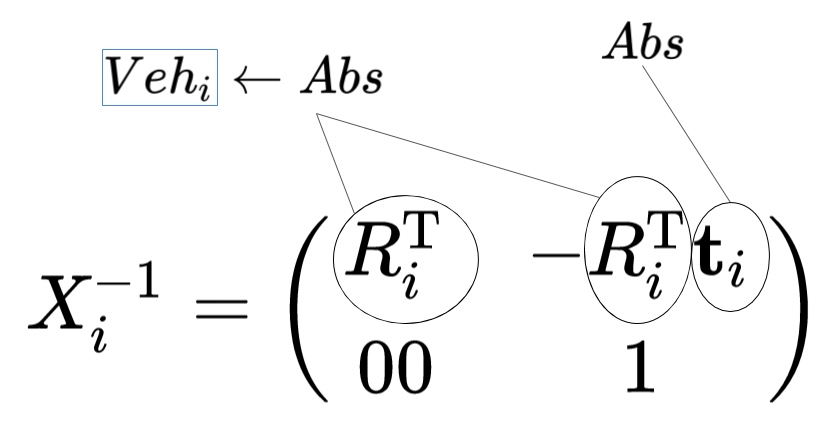
\includegraphics[width=0.4\textwidth]{2-4_pose_representation_matrix_inverse.png}
\end{figure}

\newpage

\subsection{センサーモデル}

ロボットに積載されている外界センサは、ロボットからランドマークへの距離 $d$ と角度 $\varphi$ の2つの情報を計測する。
時刻 $t_i$ と時刻 $t_j$ において同じランドマークを観測した際、それぞれの時刻で観測されたランドマークの外見の差分を取ることによって、ランドマーク自身の角度の相対的変化 $\psi_i - \psi_j$ を計算することができる。ロボットは $\psi_i$ と $\psi_j$ の絶対的な値は知ることはできず、差分を取ることでその相対値のみを知ることができる。
下記で定義する観測表現行列 $Z_{ij}$ の中にある $\theta_{ij}$ は、この各時刻で観測されたランドマーク自身の角度の差分(相対角度) $\psi_i - \psi_j$ の事を表している。

\begin{figure}[h!]
  \centering
  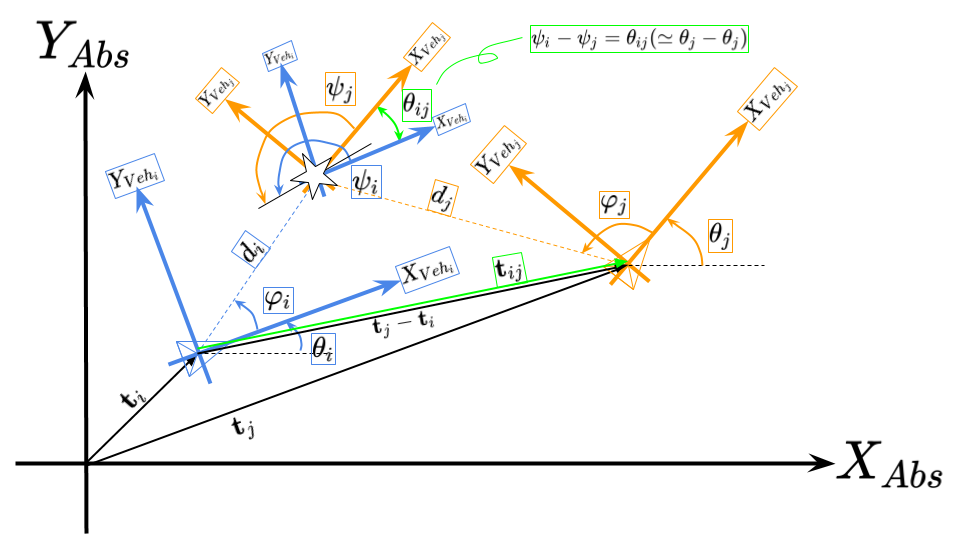
\includegraphics[width=\textwidth]{2-7_sensor_model.png}
\end{figure}

\subsection{観測表現行列: $Z_{ij}$}

違う地点から同じランドマークを観測すると、観測されたランドマークを基準にその2点間の相対的なロボットの姿勢の差を計算できる。
時刻 $t_i$ と時刻 $t_j$ において同じランドマークを観測したと仮定すると観測表現行列 $Z_{ij}$ は、

\[
Z_{ij} =
\left(
  \begin{array}{ccc}
    R_{ij} & \bm{t}_{ij} \\
       00 &              1 \\
  \end{array}
\right)
=
\left(
  \begin{array}{ccc}
    cos\theta_{ij} & -sin\theta_{ij} & x_{ij} \\
    sin\theta_{ij} &  cos\theta_{ij} & y_{ij} \\
                0 &                0 &      1 \\
  \end{array}
\right)
\]

\begin{figure}[h!]
  \centering
  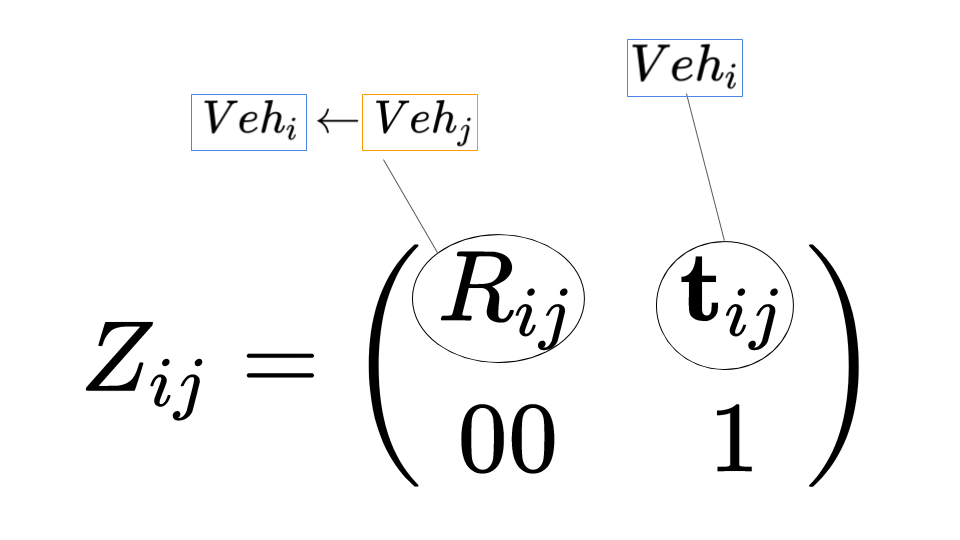
\includegraphics[width=0.4\textwidth]{2-5_observation_representation_matrix.png}
  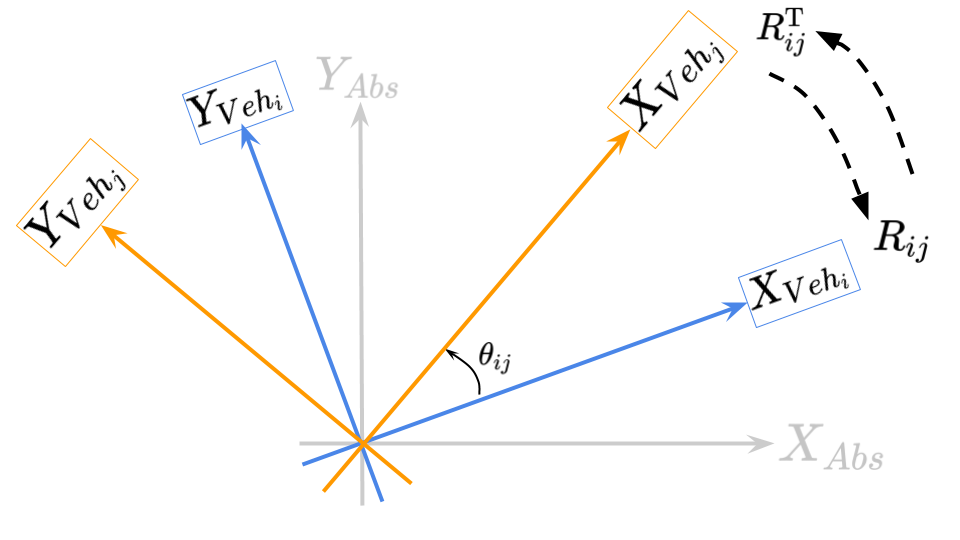
\includegraphics[width=0.5\textwidth]{2-6_rotation_matrix.png}
\end{figure}

観測表現行列 $Z_{ij}$ の原点は車両$_i$座標系上にあるので、 $\bm{t}_{ij}$ と $\theta_{ij}$ はそれぞれ車両$_i$座標系から車両$_j$座標系への距離と角度を示している。

\newpage

\section{最適化} \label{最適化}

動作辺と観測辺との誤差から計算されたコスト関数は、ガウス・ニュートン法などの最小二乗法により最適化する事ができる。

\subsection{誤差関数とコスト関数}

理想的な環境においては、観測表現行列 $Z_{ij}$ に含まれている $\bm{t}_{ij}$ と $\theta_{ij} (= \psi_i - \psi_j)$ は、各姿勢間の差 $\bm{t}_j - \bm{t}_i$ と $\theta_j - \theta_i$ にそれぞれ一致するはずである。
しかし実世界では、これらの値はセンサ誤差によって差が出てくる。この差を表したのが誤差関数 $\bm{e}_{ij}(\bm{x}_i, \bm{x}_j)$ である。

\[
\bm{e}_{ij}(\bm{x}_i, \bm{x}_j) = (\bm{x}_j - \bm{x}_i) - \bm{z}_{ij}
\]

この誤差関数 $\bm{e}_{ij}(\bm{x}_i, \bm{x}_j)$ は、前節で導入した姿勢表現行列 $X_i$, $X_j$ と、観測表現行列 $Z_{ij}$ で表現することができる。
まず、時刻 $t_i$ と時刻 $t_j$ での姿勢間の差を表す動作辺(オドメトリなど内界センサにより得られた情報)は、時刻 $t_i$ での姿勢表現行列の逆行列 $X_i^{-1}$ を時刻 $t_j$ での姿勢表現行列 $X_j$ にかける事で表現することができる。

\[
\begin{align}
X_i^{-1} X_j &=
\left(
  \begin{array}{cc}
    R_i^{\mathrm{T}} & -R_i^{\mathrm{T}}\bm{t}_i \\
                  00 &                           1 \\
  \end{array}
\right)
\left(
  \begin{array}{cc}
    R_j & \bm{t}_j \\
     00 &          1 \\
  \end{array}
\right) \\ &=
\left(
  \begin{array}{cc}
    R_i^{\mathrm{T}}R_j & R_i^{\mathrm{T}}(\bm{t}_j-\bm{t}_i) \\
                     00 &                                       1 \\
  \end{array}
\right)
\end{align}
\]

\begin{figure}[h!]
  \centering
  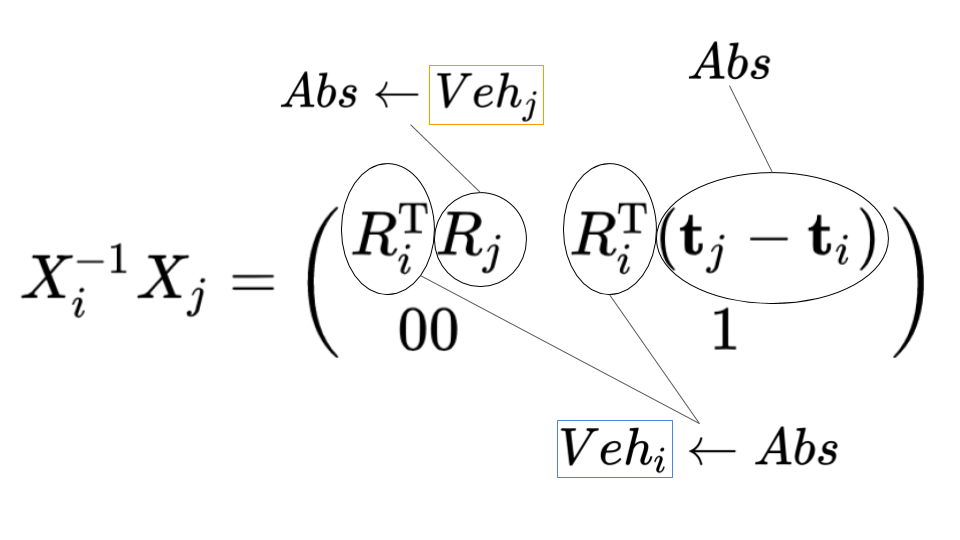
\includegraphics[width=0.5\textwidth]{3-1_difference_between_nodes.png}
\end{figure}

次に、動作辺(オドメトリなど内界センサにより得られた情報)とそれに対応する観測辺(レーザーレンジファインダなどの外界センサにより得られた情報)との間の誤差 $\bm{e}_{ij}(\bm{x}_i, \bm{x}_j)$ は、観測表現行列の逆行列 $Z_{ij}^{-1}$ をかける事で表現することができる。

\[
\begin{align}
Z_{ij}^{-1} (X_i^{-1} X_j) &=
\left(
  \begin{array}{cc}
    R_{ij}^{\mathrm{T}} & -R_{ij}^{\mathrm{T}}\bm{t}_{ij} \\
                     00 &                                 1 \\
  \end{array}
\right)
\left(
  \begin{array}{cc}
    R_i^{\mathrm{T}}R_j & R_i^{\mathrm{T}}(\bm{t}_j-\bm{t}_i) \\
                     00 &                                       1 \\
  \end{array}
\right) \\ &=
\left(
  \begin{array}{cc}
    R_{ij}^{\mathrm{T}}R_i^{\mathrm{T}}R_j & R_{ij}^{\mathrm{T}}\{R_i^{\mathrm{T}}(\bm{t}_j-\bm{t}_i)-\bm{t}_{ij}\} \\
                                        00 &                                                                            1 \\
  \end{array}
\right)
\end{align}
\]

\begin{figure}[h!]
  \centering
  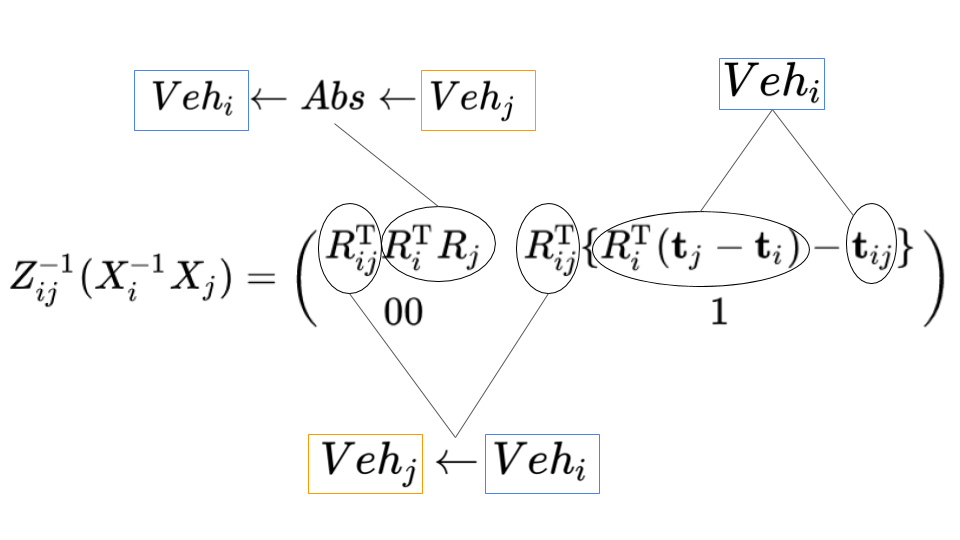
\includegraphics[width=0.6\textwidth]{3-2_error_between_edges.png}
\end{figure}

\newpage

誤差関数 $\bm{e}_{ij}(\bm{x}_i, \bm{x}_j)$ はこの行列 $Z_{ij}^{-1} (X_i^{-1} X_j)$ の平行移動要素 $R_{ij}^{\mathrm{T}}\{R_i^{\mathrm{T}}(\bm{t}_j-\bm{t}_i)-\bm{t}_{ij}\}$ と回転要素 $R_{ij}^{\mathrm{T}}R_i^{\mathrm{T}}R_j$ (の角度)によって構成されるので、

\[
\begin{align}
\bm{e}_{ij}(\bm{x}_i, \bm{x}_j) &=
\left(
  \begin{array}{cc}
    R_{ij}^{\mathrm{T}}\{R_i^{\mathrm{T}}(\bm{t}_j-\bm{t}_i)-\bm{t}_{ij}\} \\
                                   angle(R_{ij}^{\mathrm{T}}R_i^{\mathrm{T}}R_j) \\
  \end{array}
\right) \\ &=
\left(
  \begin{array}{cc}
    R_{ij}^{\mathrm{T}}\{R_i^{\mathrm{T}}(\bm{t}_j-\bm{t}_i)-\bm{t}_{ij}\} \\
                                             (\theta_j - \theta_i) - \theta_{ij} \\
  \end{array}
\right)
\end{align}
\]

グラフベースSLAMの目標は、重み付けされた二乗誤差(マハラノビス距離)と最小二乗法(ガウス・ニュートン法)を用いて、この動作辺(オドメトリなど内界センサにより得られた情報)とそれに対応する観測辺(レーザーレンジファインダなどの外界センサにより得られた情報)との間の誤差 $\bm{e}_{ij}(\bm{x}_i, \bm{x}_j)$ を最小にすることである。
この時のコスト関数は、全ての観測データにおける重み付け二乗誤差の総和である。

\[
\begin{align}
F(\bm{x}_{0:t}) &=
\sum_{i,j} \bm{e}_{ij}(\bm{x}_i, \bm{x}_j)^{\mathrm{T}} \Omega_{ij} \bm{e}_{ij}(\bm{x}_i, \bm{x}_j) \\ &=
\bm{e}_{0:t}(\bm{x}_{0:t})^{\mathrm{T}} \Omega_{0:t} \bm{e}_{0:t}(\bm{x}_{0:t})
\end{align}
\]

\subsection{線形化}

このコスト関数を最小化するのにガウス・ニュートンを用いる。
まず、誤差関数をロボットの初期経路 $\bm{x}_{0:t}$ 周りでテイラー展開し、1次近似する。

\[
\begin{align}
F(\bm{x}_{0:t} + \Delta\bm{x}_{0:t}) &=
\bm{e}_{0:t}(\bm{x}_{0:t} + \Delta\bm{x}_{0:t})^{\mathrm{T}}
  \Omega_{0:t}
    \bm{e}_{0:t}(\bm{x}_{0:t} + \Delta\bm{x}_{0:t}) \\ &\simeq
(\bm{e}_{0:t}(\bm{x}_{0:t}) + J_{0:t}\Delta\bm{x}_{0:t})^{\mathrm{T}}
  \Omega_{0:t}
    (\bm{e}_{0:t}(\bm{x}_{0:t}) + J_{0:t}\Delta\bm{x}_{0:t}) \\ &=
\{\bm{e}_{0:t}(\bm{x}_{0:t})^{\mathrm{T}} + (J_{0:t}\Delta\bm{x}_{0:t})^{\mathrm{T}}\}
  \Omega_{0:t}
    (\bm{e}_{0:t}(\bm{x}_{0:t}) + J_{0:t}\Delta\bm{x}_{0:t}) \\ &=
\bm{e}_{0:t}(\bm{x}_{0:t})^{\mathrm{T}} \Omega_{0:t} \bm{e}_{0:t}(\bm{x}_{0:t})
  + (J_{0:t}\Delta\bm{x}_{0:t})^{\mathrm{T}} \Omega_{0:t} \bm{e}_{0:t}(\bm{x}_{0:t}) \\
    &\qquad + \bm{e}_{0:t}(\bm{x}_{0:t})^{\mathrm{T}} \Omega_{0:t} (J_{0:t}\Delta\bm{x}_{0:t})
      + (J_{0:t}\Delta\bm{x}_{0:t})^{\mathrm{T}} \Omega_{0:t} (J_{0:t}\Delta\bm{x}_{0:t}) \\ &=
F(\bm{x}_{0:t})
  + \{(\Omega_{0:t}\bm{e}_{0:t}(\bm{x}_{0:t}))^{\mathrm{T}} (J_{0:t}\Delta\bm{x}_{0:t})\}^{\mathrm{T}}
    + \bm{e}_{0:t}(\bm{x}_{0:t})^{\mathrm{T}} \Omega_{0:t} J_{0:t}\Delta\bm{x}_{0:t}
      + \Delta\bm{x}_{0:t}^{\mathrm{T}}J_{0:t}^{\mathrm{T}} \Omega_{0:t} J_{0:t}\Delta\bm{x}_{0:t}
\end{align}
\]

$\Omega_{0:t}$ は対称行列、また $\bm{e}_{0:t}(\bm{x}_{0:t})^{\mathrm{T}} \Omega_{0:t} J_{0:t}\Delta\bm{x}_{0:t}$ はスカラーなので、

\[
\begin{align}
F(\bm{x}_{0:t} + \Delta\bm{x}_{0:t}) &\simeq
F(\bm{x}_{0:t})
  + (\bm{e}_{0:t}(\bm{x}_{0:t})^{\mathrm{T}} \Omega_{0:t} J_{0:t}\Delta\bm{x}_{0:t})^{\mathrm{T}}
    + \bm{e}_{0:t}(\bm{x}_{0:t})^{\mathrm{T}} \Omega_{0:t} J_{0:t}\Delta\bm{x}_{0:t}
      + \Delta\bm{x}_{0:t}^{\mathrm{T}}J_{0:t}^{\mathrm{T}} \Omega_{0:t} J_{0:t}\Delta\bm{x}_{0:t} \\ &=
F(\bm{x}_{0:t})
  + 2\bm{e}_{0:t}(\bm{x}_{0:t})^{\mathrm{T}} \Omega_{0:t} J_{0:t}\Delta\bm{x}_{0:t}
    + \Delta\bm{x}_{0:t}^{\mathrm{T}}J_{0:t}^{\mathrm{T}} \Omega_{0:t} J_{0:t}\Delta\bm{x}_{0:t} \\ &=
F(\bm{x}_{0:t})
  + 2\bm{b}_{0:t}^{\mathrm{T}} \Delta\bm{x}_{0:t}
    + \Delta\bm{x}_{0:t}^{\mathrm{T}} H_{0:t} \Delta\bm{x}_{0:t}
\end{align}
\]

ここで

\[
\bm{b}_{0:t} = J_{0:t}^{\mathrm{T}} \Omega_{0:t} \bm{e}_{0:t}(\bm{x}_{0:t}), \quad H_{0:t} = J_{0:t}^{\mathrm{T}} \Omega_{0:t} J_{0:t}
\]

\subsection{経路更新} \label{経路更新}

$\bm{x}_{0:t}$ を定数、 $\Delta\bm{x}_{0:t}$ を変数とみなすと、 $F(\bm{x}_{0:t} + \Delta\bm{x}_{0:t})$ を $\Delta\bm{x}_{0:t}$ で微分することによって、 $F(\bm{x}_{0:t} + \Delta\bm{x}_{0:t})$ を最も減らす方向の $\Delta\bm{x}_{0:t}$ を算出することができる。

\[
\frac{\partial F(\bm{x}_{0:t} + \Delta\bm{x}_{0:t})}{\partial \Delta\bm{x}_{0:t}} \simeq
2\bm{b}_{0:t} + (H_{0:t} + H_{0:t}^{\mathrm{T}})\Delta\bm{x}_{0:t} =
0
\]

$H_{0:t}$ も対称行列なので(なぜなら $\Omega_{0:t}$ が対称行列であるため)、

\[
\begin{align}
2\bm{b}_{0:t} + 2H_{0:t}\Delta\bm{x}_{0:t} &= 0 \\
\Delta\bm{x}_{0:t} &= -H_{0:t}^{-1} \bm{b}_{0:t}
\end{align}
\]

このオフセット $\Delta\bm{x}_{0:t}$ を初期経路 $\bm{x}_{0:t}$ に足し合わせることによって、最適化後のロボットの推測経路を計算することができる。

\[
\bm{x}_{0:t}' = \bm{x}_{0:t} + \Delta\bm{x}_{0:t}
\]

最後に、前回の計算結果を用いて $H_{0:t}$ と $\bm{b}_{0:t}$ を再計算し、$\Delta\bm{x}_{0:t}$ を加算して経路の更新するという上記の流れを、収束するまで\textbf{繰り返す}。

\newpage

\subsection{系全体の情報行列}

各辺の情報は、加算によって系全体の情報に反映される。
系全体の情報に加算される各辺の情報 $H_{ij}$ と $\bm{b}_{ij}$ を計算するために、誤差関数 $\bm{e}_{ij}(\bm{x}_i, \bm{x}_j)$ のヤコビアン行列 $J_{ij}$ を2つの部分行列に分ける。
誤差関数 $\bm{e}_{ij}(\bm{x}_i, \bm{x}_j)$ はロボットの各姿勢 $\bm{x}_i$ と $\bm{x}_j$ にしか依存しないので、2つに分ける部分行列の片方は $\bm{x}_i$ に関するもので、もう片方は $\bm{x}_i$ に関するものを表す。

\[
J_{ij} =
\frac{\partial \bm{e}_{ij}(\bm{x}_i, \bm{x}_j)}{\partial (\bm{x}_i,\bm{x}_j)} =
\left(
  \begin{array}{cccccc}
    \frac{\partial e_{ij_x}}{\partial x_i} & \frac{\partial e_{ij_x}}{\partial y_i} & \frac{\partial e_{ij_x}}{\partial \theta_i} & \frac{\partial e_{ij_x}}{\partial x_j} & \frac{\partial e_{ij_x}}{\partial y_j} & \frac{\partial e_{ij_x}}{\partial \theta_j} \\
    \frac{\partial e_{ij_y}}{\partial x_i} & \frac{\partial e_{ij_y}}{\partial y_i} & \frac{\partial e_{ij_y}}{\partial \theta_i} & \frac{\partial e_{ij_y}}{\partial x_j} & \frac{\partial e_{ij_y}}{\partial y_j} & \frac{\partial e_{ij_y}}{\partial \theta_j} \\
    \frac{\partial e_{ij_\theta}}{\partial x_i} & \frac{\partial e_{ij_\theta}}{\partial y_i} & \frac{\partial e_{ij_\theta}}{\partial \theta_i} & \frac{\partial e_{ij_\theta}}{\partial x_j} & \frac{\partial e_{ij_\theta}}{\partial y_j} & \frac{\partial e_{ij_\theta}}{\partial \theta_j} \\
  \end{array}
\right) =
\left(
  \begin{array}{cc}
    A_{ij} & B_{ij} \\
  \end{array}
\right)
\]

ここで $A_{ij}$ と $B_{ij}$ は、誤差関数 $\bm{e}_{ij}(\bm{x}_i, \bm{x}_j)$ をそれぞれ $\bm{x}_i$ と $\bm{x}_j$ で微分した部分行列であり、

\[
\begin{align}
A_{ij} &=
\left(
  \begin{array}{ccc}
    \frac{\partial e_{ij_x}}{\partial x_i} & \frac{\partial e_{ij_x}}{\partial y_i} & \frac{\partial e_{ij_x}}{\partial \theta_i} \\
    \frac{\partial e_{ij_y}}{\partial x_i} & \frac{\partial e_{ij_y}}{\partial y_i} & \frac{\partial e_{ij_y}}{\partial \theta_i} \\
    \frac{\partial e_{ij_\theta}}{\partial x_i} & \frac{\partial e_{ij_\theta}}{\partial y_i} & \frac{\partial e_{ij_\theta}}{\partial \theta_i} \\
  \end{array}
\right) \\ &=
\left(
  \begin{array}{ccc}
    \frac{\partial }{\partial \bm{t}_i} R_{ij}^{\mathrm{T}}\{R_i^{\mathrm{T}}(\bm{t}_j-\bm{t}_i)-\bm{t}_{ij}\} & \frac{\partial }{\partial \theta_i} R_{ij}^{\mathrm{T}}\{R_i^{\mathrm{T}}(\bm{t}_j-\bm{t}_i)-\bm{t}_{ij}\} \\
                                         \frac{\partial }{\partial \bm{t}_i} \{(\theta_j - \theta_i) - \theta_{ij}\} & \frac{\partial }{\partial \theta_i} \{(\theta_j - \theta_i) - \theta_{ij}\} \\
  \end{array}
\right) \\ &=
\left(
  \begin{array}{ccc}
    -R_{ij}^{\mathrm{T}} R_i^{\mathrm{T}} & R_{ij}^{\mathrm{T}} \frac{\partial R_i^{\mathrm{T}}}{\partial \theta_i}(\bm{t}_j-\bm{t}_i) \\
                                       00 &                                                                                             -1 \\
  \end{array}
\right) \\
\end{align}
\]

\[
\begin{align}
B_{ij} &=
\left(
  \begin{array}{ccc}
    \frac{\partial e_{ij_x}}{\partial x_j} & \frac{\partial e_{ij_x}}{\partial y_j} & \frac{\partial e_{ij_x}}{\partial \theta_j} \\
    \frac{\partial e_{ij_y}}{\partial x_j} & \frac{\partial e_{ij_y}}{\partial y_j} & \frac{\partial e_{ij_y}}{\partial \theta_j} \\
    \frac{\partial e_{ij_\theta}}{\partial x_j} & \frac{\partial e_{ij_\theta}}{\partial y_j} & \frac{\partial e_{ij_\theta}}{\partial \theta_j} \\
  \end{array}
\right) \\ &=
\left(
  \begin{array}{ccc}
    \frac{\partial }{\partial \bm{t}_j} R_{ij}^{\mathrm{T}}\{R_i^{\mathrm{T}}(\bm{t}_j-\bm{t}_i)-\bm{t}_{ij}\} & \frac{\partial }{\partial \theta_j} R_{ij}^{\mathrm{T}}\{R_i^{\mathrm{T}}(\bm{t}_j-\bm{t}_i)-\bm{t}_{ij}\} \\
                                         \frac{\partial }{\partial \bm{t}_j} \{(\theta_j - \theta_i) - \theta_{ij}\} & \frac{\partial }{\partial \theta_j} \{(\theta_j - \theta_i) - \theta_{ij}\} \\
  \end{array}
\right) \\ &=
\left(
  \begin{array}{ccc}
    R_{ij}^{\mathrm{T}} R_i^{\mathrm{T}} & \bm{0} \\
                                      00 &      1 \\
  \end{array}
\right) \\
\end{align}
\]

部分行列 $H_{ij}$ と部分ベクトル $\bm{b}_{ij}$ は $A_{ij}$ と $B_{ij}$ を用いて下記の様に書き直すことができる。

\[
H_{ij} =
\left(
  \begin{array}{cc}
    A_{ij}^{\mathrm{T}} \\
    B_{ij}^{\mathrm{T}} \\
  \end{array}
\right)
\Omega_{ij}
\left(
  \begin{array}{cc}
    A_{ij} & B_{ij} \\
  \end{array}
\right) =
\left(
  \begin{array}{cc}
    A_{ij}^{\mathrm{T}}\Omega_{ij}A_{ij} & A_{ij}^{\mathrm{T}}\Omega_{ij}B_{ij} \\
    B_{ij}^{\mathrm{T}}\Omega_{ij}A_{ij} & B_{ij}^{\mathrm{T}}\Omega_{ij}B_{ij} \\
  \end{array}
\right) \\
\]

\[
\bm{b}_{ij} =
\left(
  \begin{array}{cc}
    A_{ij}^{\mathrm{T}} \\
    B_{ij}^{\mathrm{T}} \\
  \end{array}
\right)
\Omega_{ij}
\bm{e}_{ij}(\bm{x}_i, \bm{x}_j)
=
\left(
  \begin{array}{cc}
    A_{ij}^{\mathrm{T}}\Omega_{ij}\bm{e}_{ij}(\bm{x}_i, \bm{x}_j) \\
    B_{ij}^{\mathrm{T}}\Omega_{ij}\bm{e}_{ij}(\bm{x}_i, \bm{x}_j) \\
  \end{array}
\right) \\
\]

従って系全体の情報行列 $H_{0:t}$ と系全体の情報ベクトル $\bm{b}_{0:t}$ は、これらの部分行列 $H_{ij}$ と部分ベクトル $\bm{b}_{ij}$ をそれぞれ対応する箇所に加算することで得ることができる。

\[
H_{{0:t}_{[ii]}} += A_{ij}^{\mathrm{T}}\Omega_{ij}A_{ij} \hspace{30pt}
H_{{0:t}_{[ij]}} += A_{ij}^{\mathrm{T}}\Omega_{ij}B_{ij} \\
\]
\[
H_{{0:t}_{[ji]}} += B_{ij}^{\mathrm{T}}\Omega_{ij}A_{ij} \hspace{30pt}
H_{{0:t}_{[jj]}} += B_{ij}^{\mathrm{T}}\Omega_{ij}B_{ij} \\
\]

\[
\bm{b}_{{0:t}_{[i]}} += A_{ij}^{\mathrm{T}}\Omega_{ij}\bm{e}_{ij}(\bm{x}_i, \bm{x}_j) \\
\]
\[
\bm{b}_{{0:t}_{[j]}} += B_{ij}^{\mathrm{T}}\Omega_{ij}\bm{e}_{ij}(\bm{x}_i, \bm{x}_j) \\
\]

\newpage

\section{ソースコード}

実装したソースコードの一部分を下記に示す。
$\bm{x} = (x, y, \theta)^{\mathrm{T}}$ である。

\subsection{誤差関数とコスト関数}

\begin{lstlisting}[language=python]
# Local information matrix `Omega` (from a dataset file)
Omega = edge_ij.info_matrix # 3 by 3 matrix

# Pose representation matrix `X_i` and
# Rotation matrix `R_i` on Vehicle_i coordinate
X_i = vec2mat(node_i) # 3 by 3 matrix
R_i = X_i[0:2, 0:2]   # 2 by 2 matrix

# Pose representation matrix `X_j` on Vehicle_j coordinate
X_j = vec2mat(node_j) # 3 by 3 matrix

# Observation representation matrix `Z_ij` and
# Rotation matrix `R_ij` on Vehicle_j coordinate
Z_ij = vec2mat(edge_ij.mean) # 3 by 3 matrix
R_ij = Z_ij[0:2, 0:2]        # 2 by 2 matrix

# Error between edges `e`
e = mat2vec(Z_ij.I * X_i.I * X_j) # 3 by 1 matrix
\end{lstlisting}

\subsection{線形化}

\begin{lstlisting}[language=python]
# Differentail of `R_i` ... d(R_i)/d(yaw_i)
dR_dyaw_i = np.mat([
    [-s_i, -c_i], # [-sin(yaw_i), -cos(yaw_i)],
    [c_i,  -s_i]  # [ cos(yaw_i), -sin(yaw_i)]
])
# Robot position vector `t_i`, `t_j`
t_i = node_i[0:2, 0] # 2*1 matrix, [x_i, y_i]
t_j = node_j[0:2, 0] # 2*1 matrix, [x_j, y_j]

# Separated Jacobian matrix `A_ij` which is regarding to `x_i`
A = np.mat(np.zeros((3, 3)))                     # 3 by 3 matrix with all zeros
A[0:2, 0:2] = -R_ij.T * R_i.T                    # Top left 2 by 2 elements
A[0:2, 2:3] = R_ij.T * dR_dyaw_i.T * (t_j - t_i) # Top right 2 by 1 elements
A[2:3, 0:3] = np.mat([0, 0, -1])                 # Bottom 1 by 3 elements

# Separated Jacobian matrix `B_ij` which is regarding to `x_j`
B = np.mat(np.zeros((3, 3)))    # 3 by 3 matrix with all zeros
B[0:2, 0:2] = R_ij.T * R_i.T    # Top left 2 by 2 elements
B[0:2, 2:3] = np.mat([0, 0]).T  # Top right 2 by 1 elements
B[2:3, 0:3] = np.mat([0, 0, 1]) # Bottom 1 by 3 elements

# Information sub-matrix of the system `H_ii`, `H_ij`, `H_ji`, `H_jj`
H_ii = A.T * Omega * A;    H_ij = A.T * Omega * B
H_ji = B.T * Omega * A;    H_jj = B.T * Omega * B

# Adding the sub-matrix into the information matrix of the system `H`
self.H[i_idx[0]:i_idx[1], i_idx[0]:i_idx[1]]+=H_ii;
self.H[i_idx[0]:i_idx[1], j_idx[0]:j_idx[1]]+=H_ij
self.H[j_idx[0]:j_idx[1], i_idx[0]:i_idx[1]]+=H_ji;
self.H[j_idx[0]:j_idx[1], j_idx[0]:j_idx[1]]+=H_jj

# Information sub-vector of the system `b_i`,`b_j`
b_i = A.T * Omega * e
b_j = B.T * Omega * e

# Adding the sub-vector into the information vector of the system `b`
self.b[i_idx[0]:i_idx[1]] += b_i
self.b[j_idx[0]:j_idx[1]] += b_j
\end{lstlisting}


\newpage

\subsection{経路更新}

\begin{lstlisting}[language=python]
# Add an Identity matrix to fix the first pose, `x0` and `y0`, as the origin
H[0:3, 0:3] += np.eye(3)

# Make sparse matrix of `H`
H_sparse = scipy.sparse.csc_matrix(H) # 3`n_node` by 3`n_node` matrix

# `H`^-1
H_sparse_inv = scipy.sparse.linalg.splu(H_sparse)

# `dx` = -`H`^-1 * `b`
dx = -H_sparse_inv.solve(self.b) # 3`n_node` by 1 matrix

# Reshape
dx = dx.reshape([3, self.n_node], order='F')  # 3 by `n_node` matrix

# Update
for i in range(self.n_node):
  self.node[i].pose += dx[:, i]
\end{lstlisting}

\subsection{結果}

前章\ref{経路更新}を繰り返した内の3回分を結果を以下に示す。

\begin{figure}[h!]
  \centering
  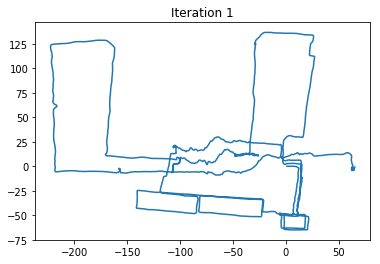
\includegraphics[width=0.4\textwidth]{4-1_by_deleji_1.png}
\end{figure}

\begin{figure}[h!]
  \centering
  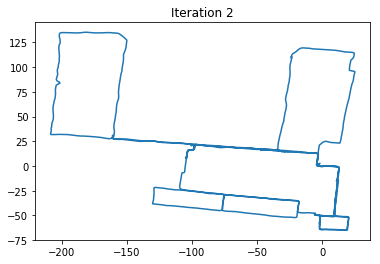
\includegraphics[width=0.4\textwidth]{4-2_by_deleji_2.png}
\end{figure}

\begin{figure}[h!]
  \centering
  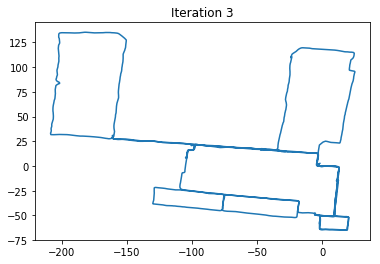
\includegraphics[width=0.4\textwidth]{4-3_by_deleji_3.png}
\end{figure}

同じ経路のはずにも関わらず違う経路だと認識されていた箇所が、元通りになっている事がわかる。

\newpage

\begin{thebibliography}{99}
  \bibitem{tutorail} G. Grisetti, R. Kummerle, C. Stachniss, and W. Burgard,
    "A tutorial on graph-based SLAM",
    IEEE Intelligent Transportation Systems Magazine,
    2010.
  \bibitem{deleji} GitHub - deleji/graph-slam: 一个二维平面的激光图优化例子,
  \url{https://github.com/deleji/graph-slam}
  \bibitem{udacity} Udacity - Artificial Intelligence for Robotics: Implementing SLAM,
  \url{https://www.udacity.com/course/artificial-intelligence-for-robotics--cs373}
\end{thebibliography}

\end{document}
